\documentclass[a4paper, 12pt, UTF8]{article}

\usepackage{xeCJK}
\setCJKmainfont[BoldFont={SimHei},ItalicFont={KaiTi}]{SimSun}

\usepackage{amsfonts}
\usepackage{amsmath}
\usepackage{graphicx}
\usepackage{indentfirst}
\usepackage{algorithm}
\usepackage{listings}
\lstset{
    columns=flexible,
    breakatwhitespace=false,
    breaklines=true,
    frame=single,
    numbers=left,
    numbersep=5pt,
    showspaces=false,
    showstringspaces=false,
    showtabs=false,
    stepnumber=1,
    rulecolor=\color{black},
    tabsize=2,
    texcl=true,
    escapeinside={\%*}{*)},
    extendedchars=false,
    mathescape=true,
}

\usepackage[colorlinks, citecolor=red]{hyperref}

\setlength{\evensidemargin}{-0.05in}
\setlength{\oddsidemargin}{-0.05in}
\setlength{\headheight}{-0.2in}
\setlength{\headsep}{0in}
\setlength{\textheight}{9.75in}
\setlength{\textwidth}{6.5in}
\setlength{\parindent}{2em}

\renewcommand{\baselinestretch}{1.5}

\begin{document}

\title{计算机视觉第3次作业}
\author{黎健成}
\date{2015210936}
\maketitle

% --------------------------------
\section{实验目的}

图像分割。


% --------------------------------
\section{实验要求}

根据课件内容,在MRF,GC,Level Set,MCMC四种方法中选择一种,参照所附文章(共八篇,每个方向2篇)完成实验。

这里选择属于Graph Cut方法的Efficient Graph-Based Image Segmentation\textsuperscript{\cite{ref1}} 文章进行实验。

% --------------------------------
\section{实验环境}

操作系统:Ubuntu 14.04.3 LTS

开发环境:gcc v4.8.5


% --------------------------------
\section{实验过程}

% ================================
\subsection{实验问题}

图像分割(Segmentation)指的是将数字图像细分为多个图像子区域(像素的集合)(也被称作超像素)的过程\textsuperscript{\cite{ref2}}。


% ================================
\subsection{实验解决方案}

这里使用Efficient Graph-Based Image Segmentation作为本次实验的解决方案。

这篇文章解决了把图像分割成区域的问题。文章定义了一个使用图像的图表示(graph-based)来衡量两个区域边界置信度的预测器,然后设计了一个基于该预测器的有效分割算法,并表明虽然该算法使用贪心决策但它产生的分割满足全局特性。文章使用2种不同的局部邻居的方法来构建图,并阐明真实与合成图像的结果。该算法的运行时间几乎与图的边数目成线性关系,在实验中也很快。该方法的一个重要特征是它能保持在变化较低的图像区域的细节,同时忽略了在变化较高的区域的细节。

\subsubsection{相关工作}

\begin{itemize}

\item 图像的图表示

图像的图表示是指将图像表达成图论中的图$G = (V, E)$。具体来说就是,把图像中的每一个像素点看成一个顶点$v_i \in V$,像素点之间的关系对(一般指相邻关系)构成图的一条边$e_i \in E$。图k 每条边的权值是基于像素点之间的关系,例如可以为像素点之间的灰度值差。

\item 最小生成树

图像用图表示之后,可以使用最小生成树方法合并像素点,使其构成若干个区域。

\end{itemize}

\subsubsection{相关定义}

\begin{itemize}

\item 分割区域(Component)的内部差(Internal difference)

假设图$G$已经简化成了最小生成树$MST(C, E)$,一个分割区域C包含若干个顶点,顶点之间通过最小生成树的边连接。这个内部差就是指分割区域C中包含的最大边的权值。
$$Int(C) = \max_{e \in MST(C, E)} w(e)$$

\item 分割区域(Component)之间的差别(Difference)

指两个分割区域之间顶点相互连接的最小边的权值。
$$Dif(C_1, C_2) = \min_{v_i \in C_1, v_j \in C_2, (v_i, v_j) \in E} w((v_i, v_j))$$
如果两个分割部分之间没有边连接,定义$Dif(C_1, C_2) = \infty$。

\item 分割区域(Component)边界的一种判断标准(predicate)

判断两个分割部分之间的差别$Dif$相对于$MInt$的大小,这里引入了一个阈值函数$\tau$ 来控制两者之间的差值。下面给出这个判断标准的定义:
$$D(C_1, C_2) = 
\begin{cases}
    \text{true}  & \text{if } Dif(C_1, C_2) > MInt(C_1, C_2) \\
    \text{false} & \text{otherwise}
\end{cases}$$
$$MInt(C_1, C_2) = \min(Int(C_1) + \tau(C_1), Int(C_2) + \tau(C_2))$$
阈值函数$\tau$主要是为了更好的控制分割区域边界的定义。比较直观的理解,小分割区域的边界定义要强于大分割区域,否则可以将小分割区域继续合并形成大区域。在这里给出的阈值函数与区域的大小有关。
$$\tau(C) = k / |C|$$
$|C|$是指分割部分顶点的个数(或者像素点个数),k是一个参数,可以根据不同的需求(主要根据图像的尺寸)进行调节。

\item 分割$S$太精细(too fine)

如果一个分割$S$,存在两个分割区域$C_1, C_2 \in S$,它们之间没有明显的边界,则称$S$太精细。

\item 分割$S$太粗糙(too coarse)

如果一个分割$S$,一个合适的调整(refinement)$S’$使得$S$不是太精细,则称$S$太粗糙。

\item 对任意一个图,都存在一个分割$S$,既不是太精细也不是太粗糙。

\end{itemize}

\subsubsection{算法过程}

算法如\textbf{Algorithm \ref{algorithm1}}所示。

\begin{algorithm}[h!]
\textbf{输入:} $n$个点、$m$条边的图$G = (V, E)$ \\
\textbf{输出:} $V$的分割$S = (C_1, \cdots, C_r)$ \\
0. 对于图$G$的所有边,按权值进行不下降排序,得到$\pi = (o_1, \cdots, o_m)$ \\
1. $S^0$是一个原始分割,相当于每个顶点当做是一个分割区域 \\
2. 重复3的操作$\text{for} q = 1, \cdots, m$ \\
3. 根据上次$S^{q - 1}$的构建。选择一条边$o_q(v_i, v_j)$,如果$v_i$和$v_j$在分割的互不相交的区域中,比较这条边的权值与这两个分割区域之间的最小分割内部差$MInt$,如果$o_q(vi, vj) < MInt$,那么合并这两个区域,其他区域不变;否则什么都不做 \\
4. 最后得到的就是所求的分割$S = S^m$
\caption{图像分割算法}
\label{algorithm1}
\end{algorithm}

\subsubsection{算法证明}

\textbf{引理1} 上述步骤3中两个通过边连接的互不相交区域,如果它们不合并,则它们将一直保留到最后。

步骤3中的边是这两个区域之间相互连接最小的边,若这条边不允许这两个区域合并,后面权值更大的边更不可能使得这两个区域合并,故这两个区域能够保留到最后。

\textbf{定理1} 通过上述算法得到的分割不是太精细。

对初始化状态$S^0$,分割是最精细的。通过算法,把能合并的区域都合并了,得到的区域之间都有明显的分界线,所以不是太精细。

\textbf{定理2} 通过上述算法得到的分割不是太粗糙。

对最后的状态$S^m$,能够合并的区域都合并了,不能合并的都保留了下来。如果对于留下来的任意一个区域进行分割,那么必然就导致这两个子区域之间没有明显的分界线,那么这个调整是太精细。显然不存在一个调整不是太精细,故最后得到分割不是太粗糙。

\textbf{定理3} 在上述算法中,相同权值的不同边的顺序不影响最后的结果。

两条边$e_1, e_2$涉及四个顶点,只有当涉及到三个区域是对实验结果可能有影响,这里只讨论这种情况。在分割区域$A$和$B$之间,在分割区域$B$和$C$之间。对$e_1$是否导致$A$和$B$合并,以及$e_2$是否导致$B$和$C$合并,分类讨论就可以很容易得出上述结论。

\subsubsection{算法效率分析}

算法使用排序和路径压缩的并查集实现,耗时主要分为两部分:

1. 步骤0的排序,使用常用的排序算法都能够达到$O(mlog(m))$。

2. 步骤1-3,时间复杂度为$O(m\alpha(m))$,$\alpha$是一个非常缓慢增长的Ackerman反函数。

主要的时间都是在第二部分,$\alpha$由于是一个增长非常缓慢的函数,所以基本可以认为是一个常数,这也是该算法基本能够与图像像素点数量成线性关系的原因。

\subsubsection{算法实现}

首先对图像进行一个高斯滤波,这样做可以去掉一些噪声,而又不影响图像的视觉效果。在构建图表示的过程采用四邻域点,即每个像素点与其周边四个像素点之间各构成一条边,边的权值通过计算颜色值的欧式距离衡量。当然也可以先在每个颜色通道进行分割,然后求它们的交,这样会使得分割效果更好(分割的更精细)。阈值函数$\tau$的参数$k$可以根据图像大小以及需求进行调节。


% ================================
\subsection{实验数据集}

\subsubsection{PASCAL VOC 2012数据集}

PASCAL VOC 2012\textsuperscript{\cite{ref3}}数据集相关地址:\url{http://host.robots.ox.ac.uk/pascal/VOC/voc2012/index.html}

PASCAL VOC(Pattern Analysis, Statistical Modelling and Computational learning, Visual Object Classes) 2012指2012年一个视觉对象的分类识别和检测的挑战赛。挑战的主要目标是识别一些现实场景中的视觉对象类。数据集中有20个分类,分别是:

\begin{itemize}

\item 人:人

\item 动物:鸟、猫、牛、狗、马、羊

\item 交通工具:飞机、自行车、船、公共汽车、汽车、摩托车、火车

\item 室内物体:瓶子、椅子、餐桌、盆栽植物、沙发、电视/显示器

\end{itemize}

比赛主要分为分类、检测、分割3个部分,这里我们只关注分割比赛。分割比赛需要对给定的物体分类生成像素级的分割,其它则作为背景。

% ================================
\subsection{实验结果}

由于这篇文章并没有实现对特定对象的分割,故没办法完成PASCAL VOC 2012中对不同对象进行分割及同一类对象不同实例的分割。这里选择几张PASCAL VOC 2012中的测试图像,使用这篇文章的分法进行实验。

图[\ref{figure_person}]、图[\ref{figure_bird}]、图[\ref{figure_aeroplane}]、图[\ref{figure_chair}]分别为4大类(人、动物、交通工具、室内物体)的图像例子及其分割结果。

\begin{figure}[h!]
    \centering
    \begin{tabular}{cc}
        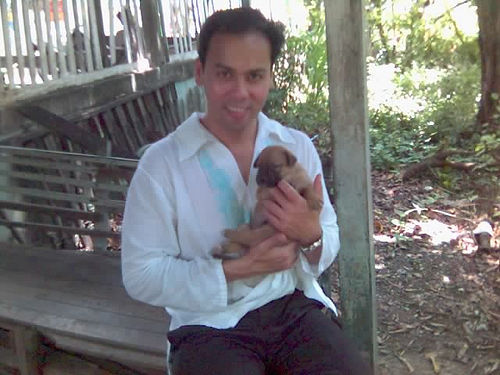
\includegraphics[width=0.4\textwidth]{src/images/2008_000026.jpg} &
        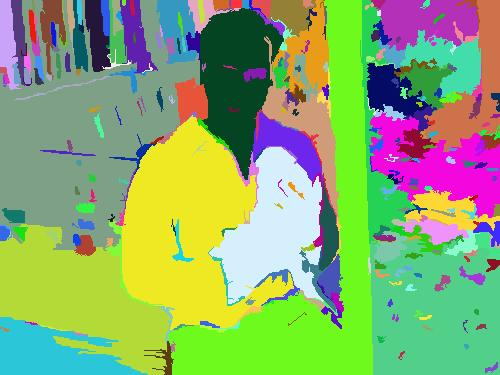
\includegraphics[width=0.4\textwidth]{src/images/2008_000026_output.jpg}
    \end{tabular}
    \caption{一张关于人的图像和它的分割结果(2008\_000026.jpg)}
    \label{figure_person}
\end{figure}

\begin{figure}[h!]
    \centering
    \begin{tabular}{cc}
        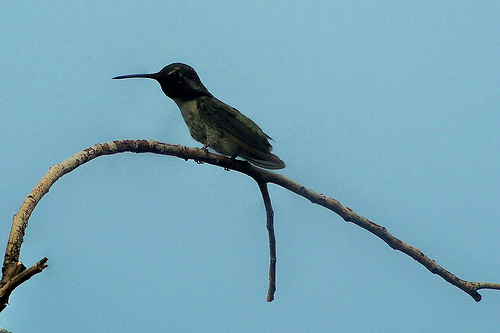
\includegraphics[width=0.4\textwidth]{src/images/2008_000123.jpg} &
        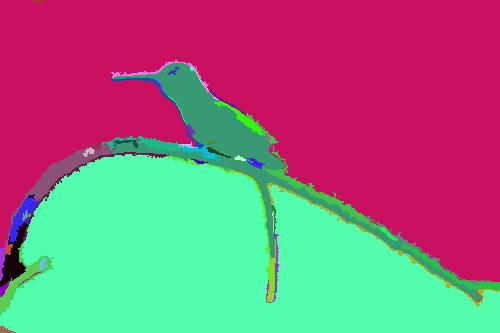
\includegraphics[width=0.4\textwidth]{src/images/2008_000123_output.jpg}
    \end{tabular}
    \caption{一张关于鸟的图像和它的分割结果(2008\_000123.jpg)}
    \label{figure_bird}
\end{figure}

\begin{figure}[h!]
    \centering
    \begin{tabular}{cc}
        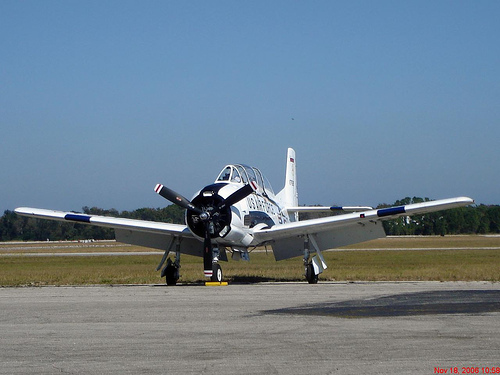
\includegraphics[width=0.4\textwidth]{src/images/2008_000021.jpg} &
        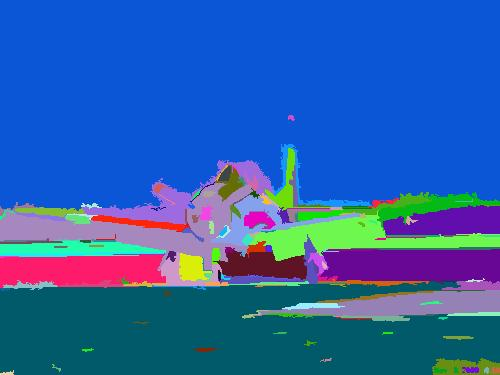
\includegraphics[width=0.4\textwidth]{src/images/2008_000021_output.jpg}
    \end{tabular}
    \caption{一张关于飞机的图像和它的分割结果(2008\_000021.jpg)}
    \label{figure_aeroplane}
\end{figure}

\begin{figure}[h!]
    \centering
    \begin{tabular}{cc}
        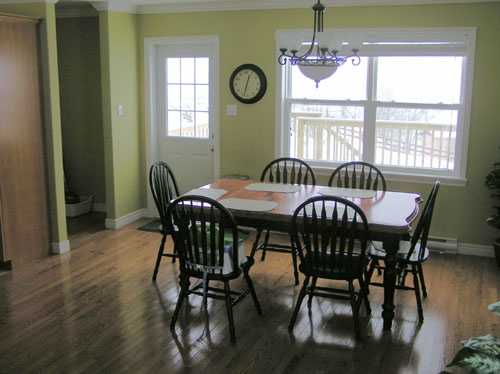
\includegraphics[width=0.4\textwidth]{src/images/2008_000043.jpg} &
        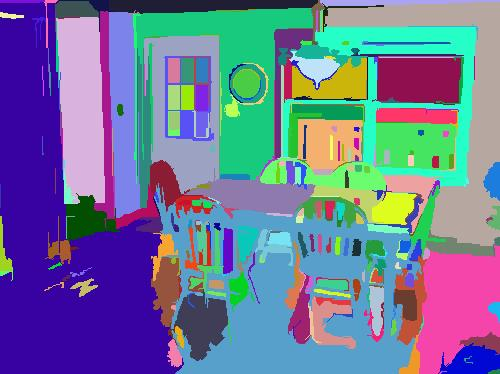
\includegraphics[width=0.4\textwidth]{src/images/2008_000043_output.jpg}
    \end{tabular}
    \caption{一张关于椅子的图像和它的分割结果(2008\_000043.jpg)}
    \label{figure_chair}
\end{figure}

% --------------------------------
\section{实验感想}

通过这次实验,熟悉了图像分割等,实现了简单的图像分割,基本达到了实验目的。


% --------------------------------
\renewcommand{\refname}{参考}
\begin{thebibliography}{9}
\bibitem{ref1} Felzenszwalb P F, Huttenlocher D P. Efficient graph-based image segmentation[J]. International Journal of Computer Vision, 2004, 59(2): 167-181.
\bibitem{ref2} 图像分割. 维基百科. 最后修订于2015年10月20日. \url{https://zh.wikipedia.org/wiki/%E5%9B%BE%E5%83%8F%E5%88%86%E5%89%B2}
\bibitem{ref3} Visual Object Classes Challenge 2012 (VOC2012).  PASCAL2. \url{http://host.robots.ox.ac.uk/pascal/VOC/voc2012/index.html}
\end{thebibliography}

\end{document}
